\chapter{Applications}

The applications of the optimal transport are many and we can find them in many discipline of sciences. Optimal couplings are used for color transferring and image segmentation, \cite{Papadakis2015OTImageProcessing}. In \cite{deGoes:2012:BNOT} is presented a way to generate high-quality blue
noise point distributions of arbitrary density functions through optimal transports. In \cite{Peyre2012TextureMixing}, Wasserstein's Barycenters are used as different way to ``average'' images. In the field of machine learning, the domain adaptation in unsupervised learning can be done with transportation plans \cite{Courty2017OTDA}. Yann Brenier, and Jean-David Benamou presented a way to compute a dynamical version of Monge-Kantorovich mass transfer problem using fluid mechanics \cite{Brenier2000Fluidmechanics}. In the field of mathematics optimal transports are studied in Riemannian manifolds \cite{Villani2008OT}, \cite{Figalli@2011}. In physics, there are many problems where optimal couplings have found a place, for example there exists a relation with Maxwellian distributions and the Monge-Kantorovich problem \cite{Tanaka1978Maxwell}. In \cite{Leonard2012Schrodinger} is presented a connection between the Kantorovich's problem and Schr\"odinger's problem, just to mention some examples among many others. \\



We present the Wasserstein's distances as an application in statistics since they can be used as a Statistical Distance between two probability distributions. As a second example we present an application of the Brenier's theorem for data assimilation of a dynamic having a linear model and a sensor. 
\section{Wasserstein's Distances as Statistical Distance.}
Optimal couplings can be used to metrize the space of probability measures. Since we can induce a distance using couplings, they are useful to use as a measure of the difference between two probability distributions, since we use already a distance of a Polish space to define it, they inherit some of the ``geometrical'' properties of the space where they are defined.  

\begin{definition}
	Let $(X,d)$ be a Polish space, and let $p\in[1,\infty)$. 
	For any two probability measures $\mu$, $\nu$ on $X$, the Wasserstein distance $\WassersteinDist{p}:\PlanSp(X)\times\PlanSp
	(X)\to\Real$ of order $p$ between $\mu$ and $\nu$ is defined by,
	\begin{equation}
		\WassersteinDist{p}(\mu, \nu)=\parentheses{\inf_{\gamma\in \Pi(\mu, \nu)}\int_{X\times X}d(x,y)^p\diff\gamma(x,y)}^{\frac{1}{p}}
	\end{equation}
	We call a Wasserstein space of order $p$ to the set, \begin{equation}
	\WassersteinSp{p}(X)=\braces{\mu\in\PlanSp(X):\quad \int_{X}d(x_0,x)\mu(\dx)<+\infty}
	\end{equation}
	where $x_0\in X$ is arbitrary. This spaces does not depend on the choice of the point $x_0$. 
\end{definition}
In words, the Wasserstein space is the space of probability measures with finite moment of order $p$. The case $p=1$ is also known as the Kantorovich distance. Since $\mu$ and $\nu$ are defined on the same space, and $d(x,y)=d(y,x)$, we see that $\WassersteinDist{p}(\mu,\nu)=\WassersteinDist{p}(\nu,\mu)$. Assume $\WassersteinDist{p}(\mu, \nu)=0$; then there exists a transport plan which is entirely concentrated on the diagonal $x=y$ in $X\times X$, therefore $\nu=\Tmeasure{\mu}{\id}$. It is possible to prove the triangle inequality, that is given $\mu_1$, $\mu_2$ and $\mu_3$, then $\WassersteinDist{p}(\mu_1,\mu_3)\leq \WassersteinDist{p}(\mu_1, \mu_2)+\WassersteinDist{p}(\mu_2, \mu_3)$. We proceed as shown in \cite{Villani2008OT} making use of the Gluing lemma and Minkowski inequality,

\begin{align}
	\WassersteinDist{p}(\mu_1, \mu_3)&=\parentheses{\int_{X\times X}d(x,z)^p\gamma_{1,3}(\dx\mathrm{dz})}^{\frac{1}{p}}\\
	&\leq\parentheses{\int_{X\times X}\parentheses{d(x,y)+d(y,z)}^p\gamma_{1,2,3}(\dx\dy \mathrm{dz})}^{\frac{1}{p}}\\
	&\leq\parentheses{\int_{X\times X}d(x,y)^p\gamma_{1,2}(\dx |\dy)\mu_2(\dy)}^{\frac{1}{p}}+\parentheses{\int_{X\times X}d(y,z)^p\gamma_{2,3}(\dy| \mathrm{dz})\mu_3(\mathrm{dz})}^{\frac{1}{p}}\\
	&\leq\parentheses{\int_{X\times X}d(x,y)^p\gamma_{1,2}(\dx \dy)}^{\frac{1}{p}}+\parentheses{\int_{X\times X}d(x,z)^p\gamma_{2,3}(\dx|\mathrm{dz})}^{\frac{1}{p}}\\
	&=\WassersteinDist{p}(\mu_1,\mu_2)+\WassersteinDist{p}(\mu_2,\mu_3)
\end{align} 
We can find a more structured proof for the triangle inequality in \cite{Santambrogio2015OT} in the section of Wasserstein Spaces.
Note that the inequality, 
\begin{equation}
	d(x,y)\leq 2^{p-1}\left(d(x, x_0)^p+d(x_0, y)^p\right)
\end{equation}
shows that $\WassersteinDist{p}$ is finite on $\WassersteinSp{p}$, since $\WassersteinDist{p}(\mu,\nu)\leq 2^{p-1} \parentheses{\int_{X}d(x, x_0)^p\dmu(x)+\int_{X}d(x, x_0)^p\dnu(x)}<\infty$.

In the following we just state some interesting topological results in $\WassersteinSp{p}$ spaces that have implications in several applications, the reader can find the respective proofs in \cite{Villani2008OT},
\begin{definition}[Weak Convergence in $\WassersteinSp{p}$]
	Let $(X,d)$ be a Polish space, and $p\in[1,\infty)$. Let $(\mu_k)_{k\in\Naturals}$ be a sequence of probability measures in $\WassersteinSp{p}(X)$ and let $\mu$ be another element of $\WassersteinSp{p}(X)$. Then $(\mu_k)_{k\in\Naturals}$ is weakly convergent in $\WassersteinSp{p}(X)$ if any one of the following properties is satisfied for any $x_0\in X$:
	\begin{itemize}
		\item $\mu_k\rightarrow \mu$ and $ \int_{X} d(x_0, x)^p \diff\mu_k(x)\rightarrow \int_{X}d(x_0, x)^p\diff\mu(x);$
		\item $\mu_k\rightarrow \mu$ and $\limsup_{k\rightarrow \infty}\int_{X} d(x_0, x)^p\diff\mu_k(x)\leq \int_{X}d(x_0, x)^p\diff\mu(x)$
		\item $\mu_k\rightarrow \mu$ and $\lim_{R\rightarrow \infty}\limsup_{k\rightarrow \infty} \int_{d(x_0,x)\geq R} d(x_0, x)^p\diff\mu_k=0$
		\item For all continuous functions $\phi$ with $\abs{\phi}\leq C(1+d(x_0, x)^p)$, $C\in \Real$, one has
		\begin{equation}
			\int\phi(x)\diff\mu_k(x)\rightarrow \int\phi(x)\diff\mu(x)
		\end{equation}
	\end{itemize}
\end{definition}
\begin{theorem}
	Let $(X,d)$ be a Polish space, and $p\in[1,\infty)$; then the Wasserstein distance $\WassersteinDist{p}$ metrizes the weak convergence in $\WassersteinSp{p}$. That is, if $(\mu_k)_{k\in\Naturals}$ is a sequence of measures in $\WassersteinSp{p}$ and $\mu$ is another measure in $\PlanSp(X)$, then, the statement $\mu_k$ converges weakly in $\WassersteinSp(X) $ to $\mu$ and $\WassersteinDist{\mu_k,\mu}\rightarrow 0$ are equivalent.  
\end{theorem}
If $(X, d)$ is a Polish space, and $p\in[1,\infty)$, the $\WassersteinDist{p}$ is continuous on $\PlanSp(X)$. Explicitly if $\mu_k$(respect to $\nu_k$) converges to $\mu$ weakly (respect to $\nu$ ) in $\WassersteinSp{p}$ as $k\rightarrow \infty$ then $\WassersteinDist{p}(\mu_k, \nu_k)\rightarrow \WassersteinDist{p}(\mu, \nu)$. The Wasserstein distance is lower semicontinuous on $\PlanSp(X)$. If $\tilde{d}$ is a bounded distance inducing the same topology\footnote{For example $\tilde{d}=\frac{d}{1+d}$. Check \cite{munkres2000topology} for the proof that $\tilde{d}$ is bounded and induces the same topology.} as $d$, then the convergence in Wasserstein sense for the distance $\tilde{d}$ is equivalent to the usual weak convergence of probability measures in $\PlanSp(X)$. Any Cauchy Sequence in $\WassersteinSp{p}$ is tight.
\\
The definition of Wasserstein distances makes them convenient to use in problems related with optimal transport, specially many problems coming from partial differential equations.

To conclude this section we  introduce the Wasserstein Barycenter problem.
\begin{problem}
	Let $X$ a Polish space, and let $\mu_1, \mu_2, \dots, \mu_n$ a set of probability measures defined on $X$. Find $\tilde{\mu}\in \WassersteinSp{p}$, such that
	\begin{equation}
		\sum_{i=1}^{n}\WassersteinDist{p}(\tilde{\mu}, \mu_i)\leq \sum_{i=1}^{n}\WassersteinDist{p}(\mu,\mu_i),\quad \forall \mu \in \WassersteinSp{p}(X).
	\end{equation}
	That is find the measure $\mu$ that is closer in average to all the given measures in the sense of  $\,\WassersteinSp{p}$ metric.
\end{problem}

%\section{Data Assimilation of a Dynamic.}
%\section{Isoperimetric Inequality.}
%\section{Dynamical Optimal transport.**}
\section{Track of a Dynamic (Kalman Filter).}
An interesting application of optimal transport is the design of filters for data taken from noisy environments.	
For the sake of simplicity consider an dynamical system,
\begin{align}
\mathbf{x}_{n+1}=\mathbf{A}\,\mathbf{x}_{n}+\mathbf{B}u_n
\end{align}
where $\mathbf{x}_n\in\Real^n$ is a time series vector constrained to the dynamic given by the constant matrices $\mathbf{A}\in\mathbf{M}^{n\times n}$, $\mathbf{B}\in \mathbf{M}^{n\times m}$ and a control variable $\mathbf{u}_n\in\Real^n$. 

The above equation is just an idealization of the reality, usually the models ignore small perturbations in order to have a simple and useful model that describes the reality without getting too far from it, as Einsteins says: ``Everything should be as simple as possible but not simpler''. In practice, many models satisfy this condition, therefore we can assume that the original state $\mathbf{y}_n$ is not the ideal state but behaves really similar. It is reasonable to consider $\mathbf{y}$ as the ideal state plus some noise\footnote{Please note that this is an assumption, in many applications this models in good way the phenomenon. Although there is a huge set of problems that this approach result flawed or insufficient.}. For the sake of simplicity, we find convenient to consider it as a random variable normally distributed $\mathbf{y}_n\sim\mathcal{N}(\mathbf{x}_n,\pmb{\Sigma}_x)$ with expected value $\mathbf{x}_n$ and a covariance matrix $\pmb{\Sigma}_x$.

Imagine we are trying to read the data from the original state $\mathbf{y}_n$ using a sensor. In practice, the environment is noisy and sensors are not perfect. This conditions get reflected as noise in the acquisition of data. We can consider the data obtained from the sensor as a random variable normally distributed $\mathbf{z}_n$ with expected value $\mathbf{y}_n$, without loss of generality this is equivalent to say $\mathbf{z}_n=\mathbf{y}_n+\pmb{\sigma}$, where $\pmb{\sigma}$ is a random variable normally distributed with zero mean and covariance matrix $\pmb{\Sigma}_z$. 
	
We remark that are able to read the sensor, so we would like to find a joint probability measure that given a reading of the sensor allows to predict the next state of the dynamic as close as possible. 

We need to choose a measure for the difference between the prediction and reality. For simplicity we choose a standard deviation. This is nothing less that an optimal transport formulation of the problem, with the marginals given by normal distributions of our two random variables and a cost function $c(x,y)=\abs{x-y}^2$.  Moreover, from the Brenier's theorem we know that this joint probability measure is a deterministic coupling given by a map $T$.
Hence we reduce it to an optimal map problem, 
\begin{align}
\min_{T}\mathbb{E}\brackets{\norm{\mathbf{y}_{n+1}-T(\mathbf{z}_n)}^2}\\
\subject \, \nu = \Tmeasure{\mu}{T}
\end{align}
where $\mu$ and $\nu$ are the normal distributions corresponding to the random variables $\mathbf{z}_n$ and $\mathbf{y}_{n+1}$ respectively. Both variables are normally distributed, and the cost function is the squared euclidean distance, therefore the $T$ is an affine map given by,

\begin{align}
	T(\mathbf{z}_{n})=\mathbf{x}_{n}+\pmb{\Sigma}\mathbf{A}^{\top}\pmb{\Sigma}_z^{-1}\parentheses{\mathbf{z}_n-\mathbf{A}\mathbf{x}_{n}}\\
	\text{where, }\pmb{\Sigma}=\parentheses{\mathbf{A}^\top \pmb{\Sigma}_z^{-1}\mathbf{A}+\pmb{\Sigma}_x^{-1}}^{-1} \nonumber
\end{align}

The above equation is the map generating a deterministic coupling between a normally distributed random variable under a linear map and an arbitrary random variable that is also normally distributed. Please check \cite{Tarek2012OTFilter} and \cite{Dean2014OTFilters} for a detailed derivation of the equations. 

Please note that computing this map is not possible, since we need the ideal state and this is something that we are not able to obtain, even if our sensor is perfect. Although, we can do an approximation. We proceed as Kalman did in the development of the filter bearing his name.\\

We start with a guess of the initial state, $\mathbf{r}_0$ and we read our first sample from the sensor $\mathbf{z}_0$, we use our initial guess to do an approximation of the ideal state, that is $\mathbf{x}_{0}\approx \mathbf{A}\mathbf{r}_0+\mathbf{B}\mathbf{u}_0=\tilde{\mathbf{x}}_0$. And we save $\mathbf{r}_{1}=T(z_{0})$ since we consider that this is the best approximation we can get from the dynamic under standard deviation measure. We continue in this way, taking a sample from the sensor and using the data to get good approximations $\tilde{\mathbf{x}}_{n+1}=\mathbf{A}\,\mathbf{r}_n+
\mathbf{B}\mathbf{u}_n$ of the reality, 

\begin{align}
T(\mathbf{z}_{n})&=\tilde{\mathbf{x}}_{n}+\pmb{\Sigma}\mathbf{A}^{\top}\pmb{\Sigma}_z^{-1}\parentheses{\mathbf{z}_n-\mathbf{A}\tilde{\mathbf{x}}_n}\\
\mathbf{r}_{n+1}&=T(\mathbf{z}_n)
\end{align}

If our assumptions are consistent with the reality $\mathbf{r}_n$ is the best approximation we can do sampling $\mathbf{z}_{n-1}$ from the sensor  at step $n-1$, and our filtered data should not be far from the reality.


As example consider the circuit shown in figure \ref{fig: RLC circuit} whose dynamic is given by,
\begin{align}
\begin{bmatrix}
\dot{x}_1\\ \dot{x}_2
\end{bmatrix}=\begin{bmatrix}
0&1/(RC)\\
-R/L & -R/L
\end{bmatrix}\begin{bmatrix}x_1\\ x_2\end{bmatrix}+\begin{bmatrix}0\\R/L\end{bmatrix} v_{in}=A_cx+Bv_{in}
\end{align}
In this hypothetical situation consider that the sensor is able to take samples at a frequency of $10$kHz, that is a sampling period $T=$1e-4 seconds and the source $v_{in}=\sin(2\pi f t)$, where $f=100$Hz. The values for the electrical components are $R=1$k$\Omega$ for the resistance, $L=100$m$H$ for the inductance, and $C=1$e-6F for the capacitance. The discrete version of this dynamic is given by,
\begin{equation}
	\mathbf{x}_{n+1}=\begin{bmatrix}
		0,9056542 & 0,0009066\\
		−0,9065617 & −0,0009075
	\end{bmatrix}\mathbf{x}_{n}+\begin{bmatrix}
	0,0943458\\
	0,9065617
	\end{bmatrix}u_{n}
\end{equation}
The above equation was obtained using the equations,
\begin{equation}
	\mathbf{A}=\mathsf{e}^{A_c T}, \quad \mathbf{B}=A_c^{-1}(\mathbf{A}-\mathbf{I})B,
\end{equation}
and $u_n$ is just the sample of the input $v_in$ at time $nT$ corresponding to the $n$ sample, i.e. $u_n=\sin(2\pi fnT)$.
\begin{figure}[H]
	\begin{subfigure}{0.48\textwidth}
		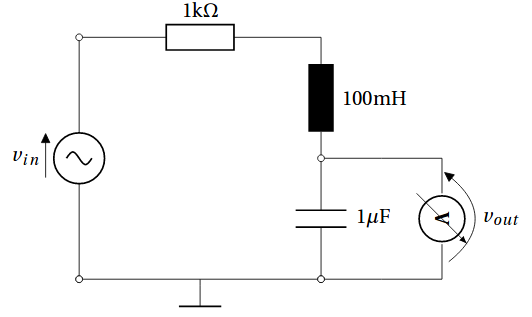
\includegraphics[width=0.95\textwidth]{RLC}
		\caption{RLC Circuit.} 
		\label{fig: RLC circuit}
	\end{subfigure}
	\begin{subfigure}{0.45\textwidth}
		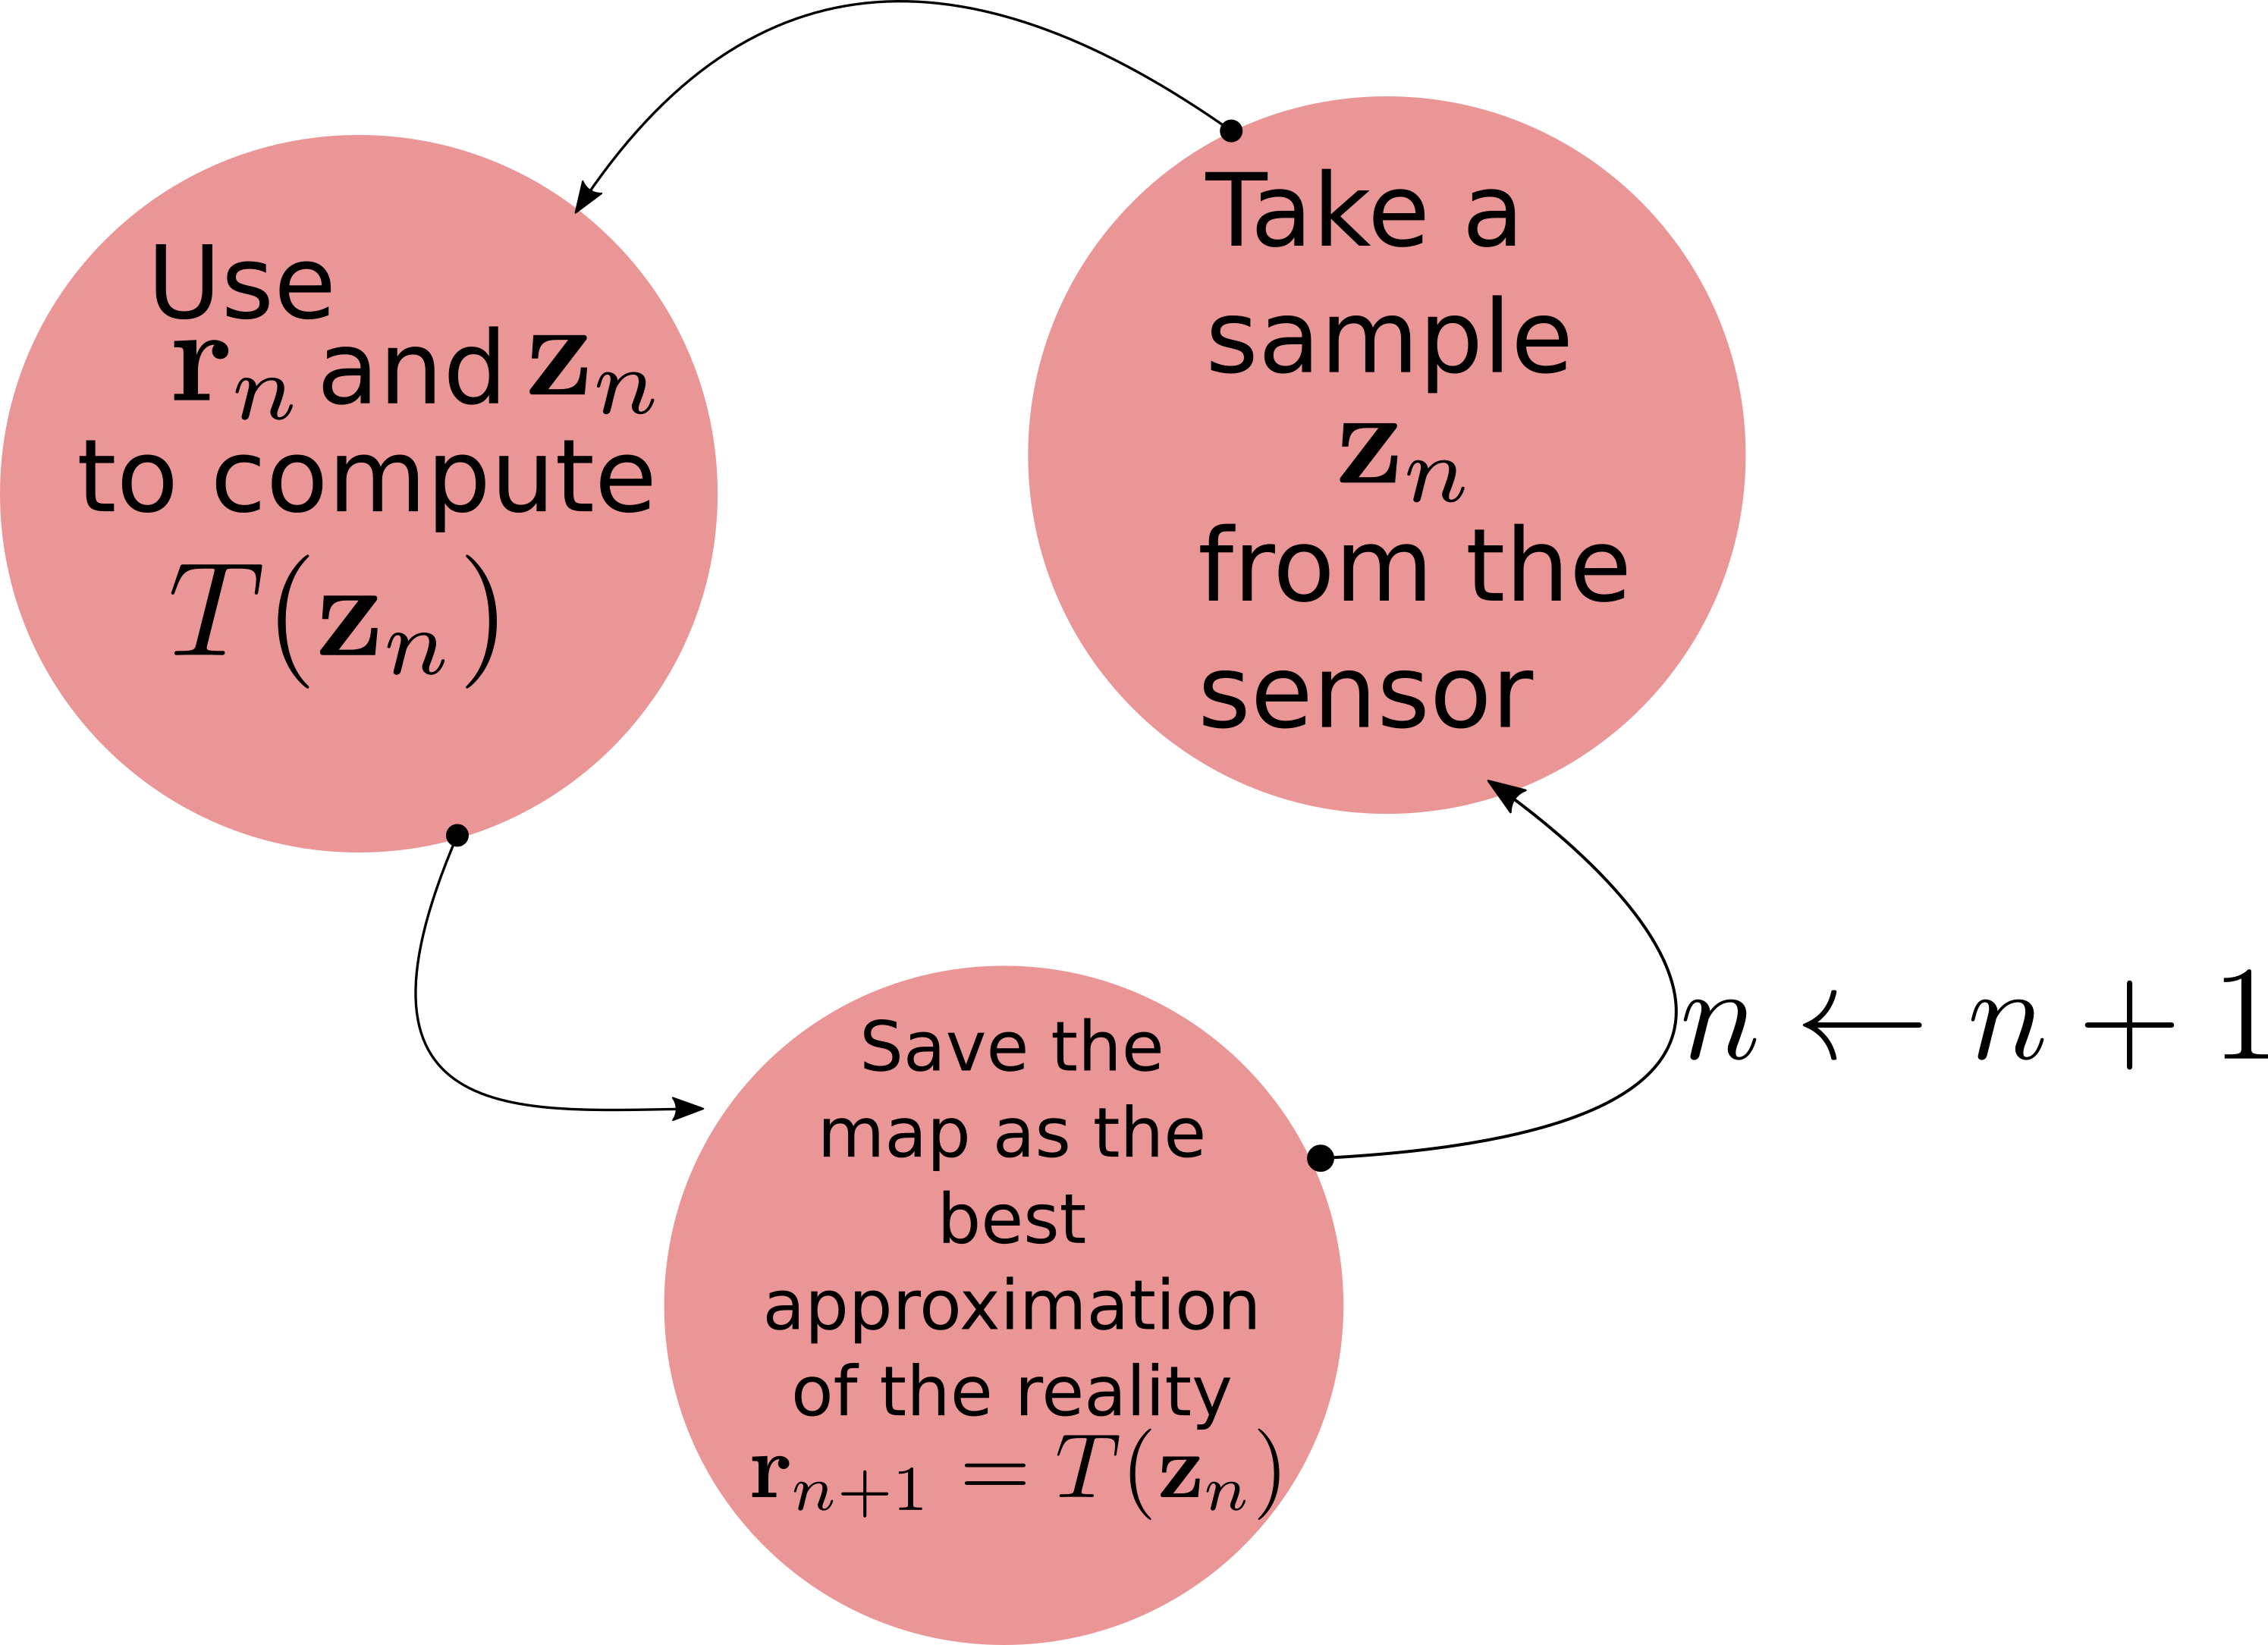
\includegraphics[width=0.75\textwidth]{FilterOTAlg}
		\caption{Procedure to track a dynamic.}
	\end{subfigure}
\end{figure} 
The figure \ref{fig: Graphs.} shows the results obtained for the described dynamical system. Note that we have two simulations, one for an initial guess equal to the ideal state and one for an initial guess totally different to the ideal state. We can appreciate that even if we started from a bad guess for the initial state, the coupling works properly.
\begin{figure}[H]
	\begin{center}
	\caption{Filter with Optimal Transport coupling. $\pmb{\Sigma}_z=0.2$, $\pmb{\Sigma}_x=0.01$.}		
	\label{fig: Graphs.}
	\begin{subfigure}{0.48 \textwidth}
	\caption{Initial guess $\mathbf{r}_0=\mathbf{x}_0$}
	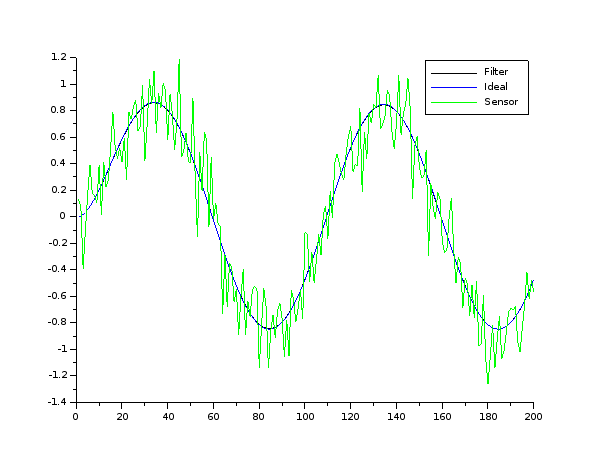
\includegraphics[width=0.98\textwidth]{OTFilter}
	\end{subfigure}
	\begin{subfigure}{0.48\textwidth}
	\caption{Initial guess $\mathbf{r}_0\neq\mathbf{x}_0$}
	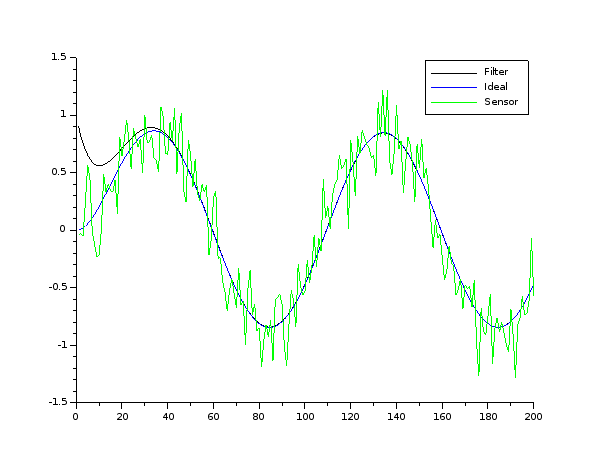
\includegraphics[width=0.98\textwidth]{OTFilter2}
	\end{subfigure}
	\end{center}

\end{figure}
%\section{Applications in Image Recognition.**}
%\section{Barycenter of a Fourier Power Spectrum.****}
%\section{Approximation of Euler Equations.}
%\section{Nash Equilibrium.}
%\section{Track of a Dynamic.}